\documentclass[]{beamer}

\usepackage[style=authoryear]{biblatex}
\usepackage{hyperref}

\usepackage[font=small]{caption}
\usepackage{booktabs}
\usepackage{tabularx}
\newcolumntype{Y}{>{\raggedright\arraybackslash}X}
\newcolumntype{s}{>{\raggedright\arraybackslash\hsize=.5\hsize}X}
\AtBeginEnvironment{tabularx}{\tiny}
\usepackage{xltabular}
\AtBeginEnvironment{xltabular}{\tiny}

\addbibresource{mainstream.bib}

\usetheme{CambridgeUS}
\usecolortheme{beaver}

\title[How has Mainstream changed?]{How has Mainstream changed? \\ \small A Topic Model insight}
\author[Ciruzzi, M.]{Michele Ciruzzi}
\institute[UnInsubria]{Università degli Studi dell'Insubria}

\date{2023 ESHET Conference}

\begin{document}

\frame{\titlepage}

\section{Why studying the mainstream?}
\begin{frame}
	\frametitle{Why studying the top journals}
	Economics presents very strong social norms and a very hierarchical structure.

	The scholars in the top US departments publish in small group of journals \parencite{card2013,kim2006,kim2009,dusansky1998,hamermesh2013,ellison2003,heck2006}.

	Those same journals can assure a scholar the tenure in the very same departments \parencite{heckman2020}.
\end{frame}

\section{Research questions}
\begin{frame}
	\frametitle{The empirical turn}
	The first lens with which to observe the mainstream economics is the progressive shift toward empirical research \parencite{backhouse2000,backhouse2016,backhouse2017,cherrier2022}.

	Econometrics is becoming the standard mathematical tool of analysis and theory-driven models are being replaced by data-driven models.
\end{frame}

\begin{frame}
	\frametitle{The mainstream pluralism}
	The second lens is the mainstream pluralism hypothesis \parencite{davis2006,davis2019a,davis2019b,cedrini2018}.

	The domain of research of economics is widening and the number of different computational and mathematical tools used is increasing.

	These two tendencies have allowed the emergence of many new fields in the discipline, which are very focused on a particular topic (like environmental or health economics) or on a particular method (like economic complexity or experimental economics).
\end{frame}

\section{Methods and Data}
\begin{frame}
	\frametitle{Distant Reading}
	Distant Reading \parencite{moretti2013}: instead of carefully (close) reading few works, a big number of documents are summarily analysed using statistical methods and the aid of computers.

	Different features of a text can be analysed, but generally the focus is on the textual content of the document (recovered by a digital version or through OCRing) or some metadata (title, citations, authors' list).
\end{frame}

\begin{frame}
	\frametitle{The Journals}
	\begin{enumerate}
		\item The American Economic Review
		\item Econometrica
		\item Journal of Political Economy
		\item Quarterly Journal of Economics
		\item Review of Economic Studies
		\item Review of Economics and Statistics
		\item Economica
		\item The Economic Journal
	\end{enumerate}
\end{frame}

\begin{frame}
	\frametitle{Timespan}
	The research article published between 1946 (the first year after the WWII) and 2016 (the last year for which the full-texts of the articles was available for the eight journals in the sample) are considered.
\end{frame}

\begin{frame}
	\frametitle{Bag-of-Words}
	Bag-of-Words (BoW) approximation: the corpus is represented as a matrix with the documents on the rows, the different words on the columns, and the frequencies as entries.

	The same matrix represents also a bipartite graph and a linear space of documents spanned by the words.
\end{frame}

\begin{frame}
	\frametitle{Hierarchical Stochastic Block Model (hSBM)}
	\begin{figure}
		\centering
		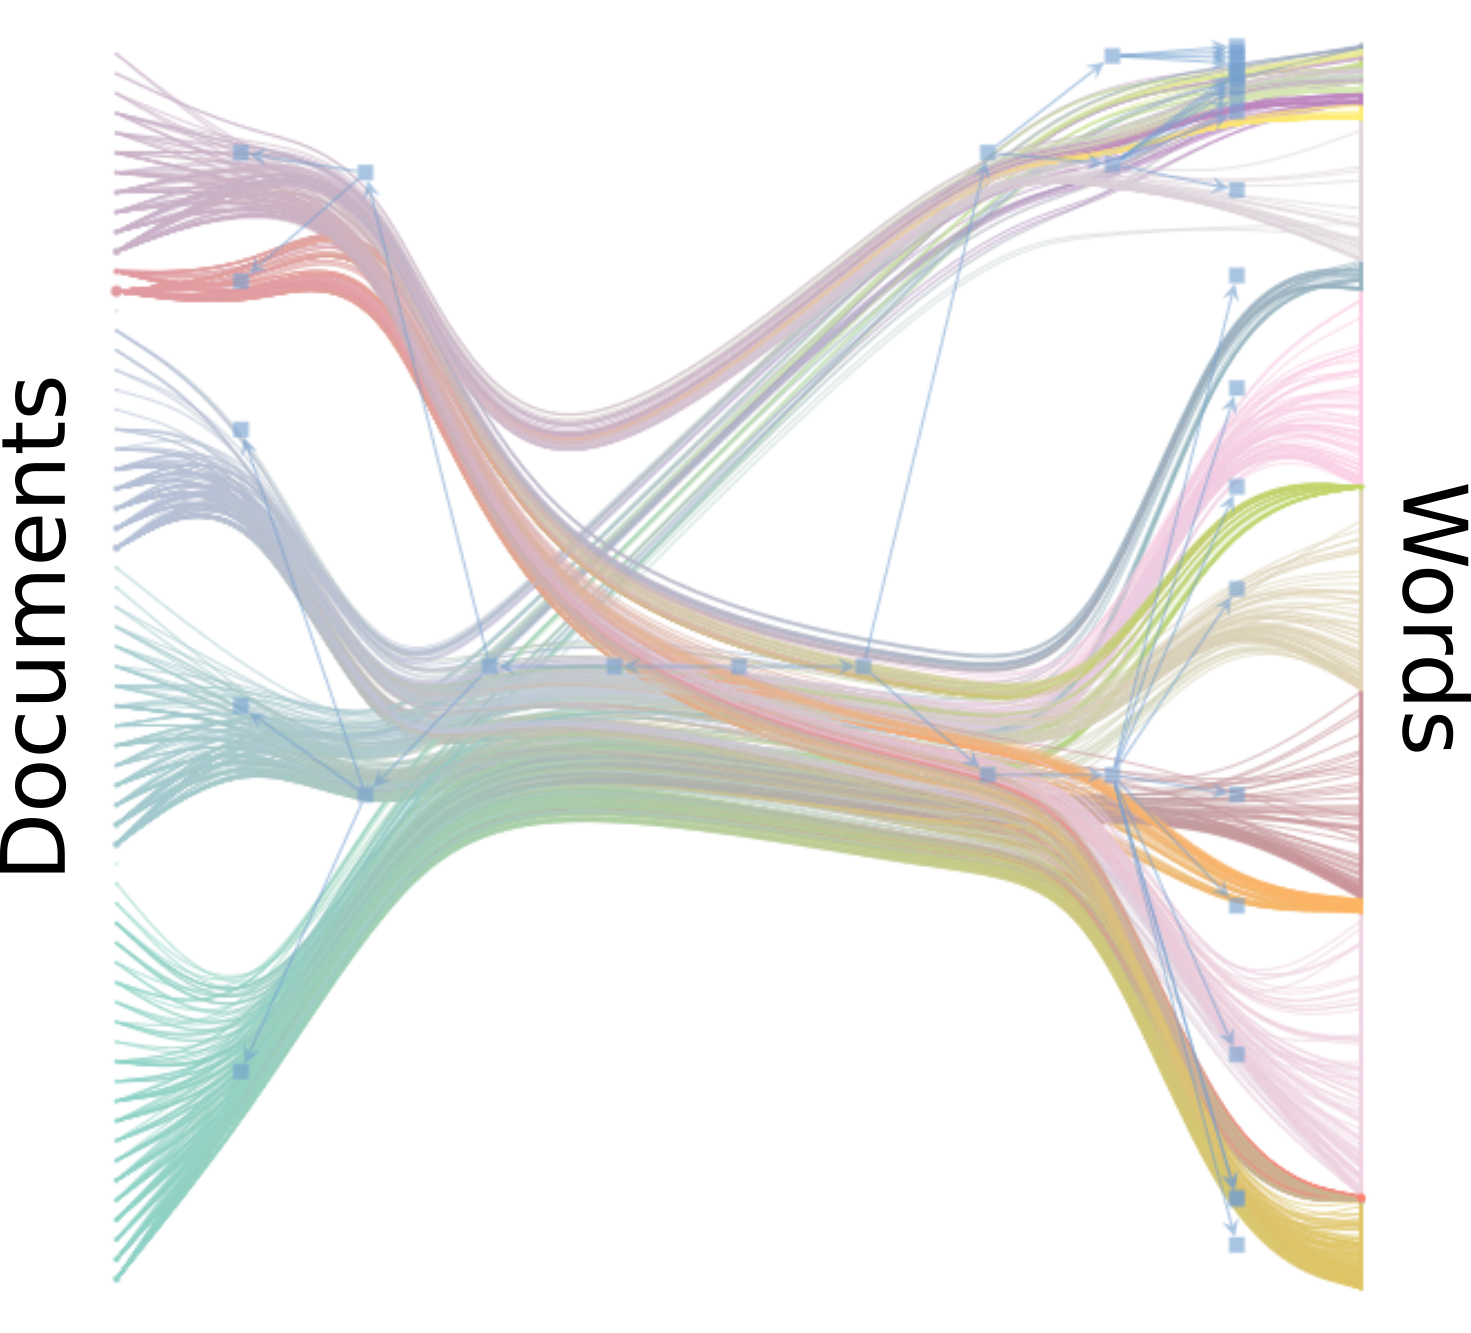
\includegraphics[width=.45\linewidth]{slide_src/bipartite.png}
		\caption{An example of resulting graph (source: \url{https://topsbm.github.io/})}
	\end{figure}
\end{frame}

\begin{frame}
	\frametitle{Dataset composition}
	The documents are lowercased, tokenized and stemmed.

	Only the words which appear in at least 35 documents (approximately 1 every 1000) and at most in 9000 documents (approximately one fourth of the corpus) are kept.

	\begin{table}[tb]
\caption[Dataset size]{Number of documents, unique words and tokens in the dataset at three different stages of the cleaning process}
\label{tab:dataset}
\begin{tabular}{l|rrr}
\toprule
 & Documents & Words & Tokens \\
\midrule
Original dataset & 81309 & 10323373 & 438722824 \\
After first cleaning & 35513 & 2040481 & 178900475 \\
Final dataset & 32985 & 32520 & 38041150 \\
\bottomrule
\end{tabular}
\end{table}

\end{frame}

\begin{frame}
	\frametitle{Dataset composition}
	\begin{figure}
		\centering
		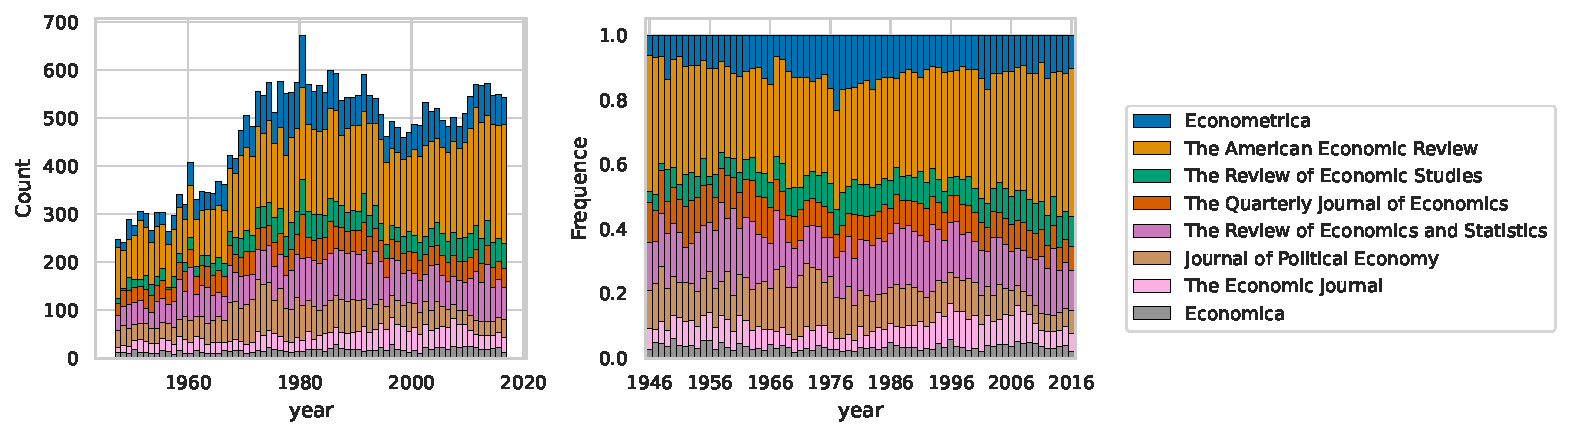
\includegraphics[width=\textwidth]{src/journals.pdf}
		\caption[Number of documents per journal and year]{These two plots represent the number of documents in the dataset divided by year and journal. On the left, the absolute number is reported, while on the right the same data are reported normalized by year.}
	\end{figure}
\end{frame}

\section{Results}
\begin{frame}
	\frametitle{Robustness of the algorithm}
	\begin{table}[tb]
\caption[Number of groups per level and seed]{Number of groups (both words and documents) in each level of the hierarchy for each random seed}
\label{tab:levels}
\begin{tabular}{l|rrrrrr}
\toprule
level & 0 & 1 & 2 & 3 & 4 \\
seed &  &  &  &  &  \\
\midrule
1000 & 1369 & 185 & 32 & 5 & 2 \\
1001 & 1207 & 179 & 26 & 5 & 2 \\
1002 & 1494 & 193 & 34 & 6 & 2 \\
1003 & 4288 & 479 & 64 & 11 & 2 \\
1004 & 1508 & 312 & 57 & 8 & 2 \\
\bottomrule
\end{tabular}
\end{table}

\end{frame}

\begin{frame}
	\frametitle{Robustness of the algorithm}
	\begin{figure}
		\centering
		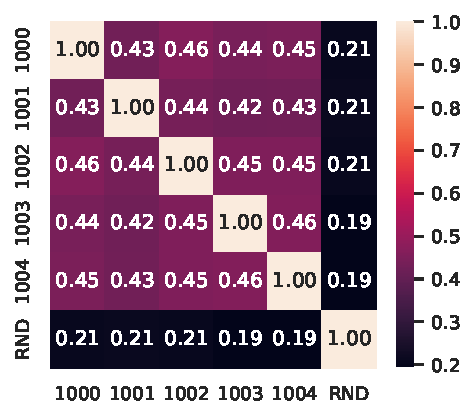
\includegraphics[width=2.5in]{src/mi.pdf}
		\caption[Mutual Information for the level of interest]{Normalized mutual information for the three level 3 partitions and a random control partition (RND)}
	\end{figure}
\end{frame}

\begin{frame}
	\frametitle{Groups}
	\begin{table}[tb]
\caption[Groups]{The nine documents-group and the twenty most frequent words in each of them}
\label{tab:groups}
\begin{tabularx}{\hsize}{lY}
\toprule
\midrule
Game Theory & des, les, tariff, export, que, plant, bargain, debt, est, shock, foreign, par, union, dan, domest, pour, une, entri, manufactur, agreement \\
Production & household, unemploy, educ, game, shock, inflat, export, job, player, foreign, labour, union, hous, panel, insur, credit, match, payoff, hour, debt \\
\bottomrule
\end{tabularx}
\end{table}

\end{frame}

\begin{frame}
	\frametitle{Groups}
	\begin{figure}
		\centering
		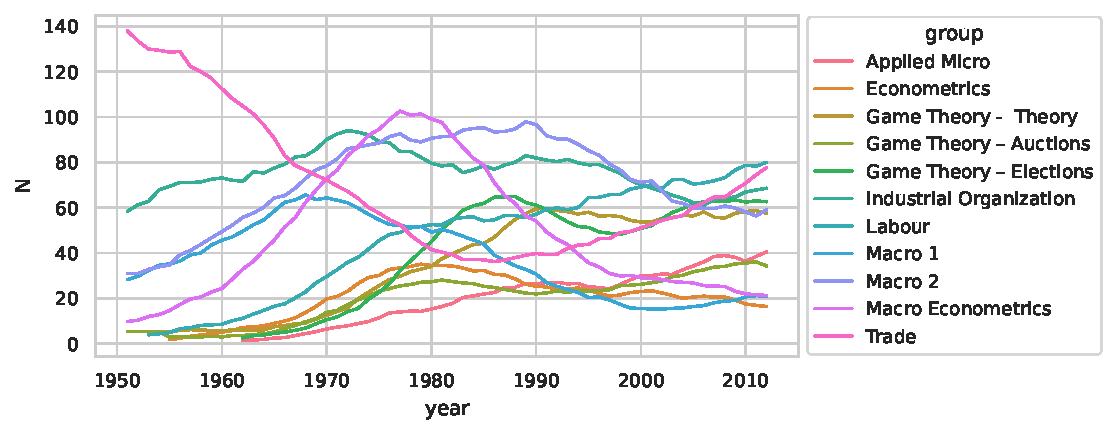
\includegraphics[width=\textwidth]{src/groups.pdf}
		\caption[Groups]{Number of documents in each group during time. Smoothed with a 10-year rolling average}
	\end{figure}
\end{frame}

\begin{frame}
	\frametitle{Topics}
	\vspace{-1.5em}
	\begin{table}[tb]
\caption[Topics]{The twelve topics (words-group) and the twenty most frequent words for each of them}
\label{tab:topics}
\begin{tabularx}{\hsize}{lY}
\toprule
\midrule
Anti-Trust & cartel, herd, franchis, cascad, barrel, boycott, fad, ivo, sushil, conspir, lusion \\
Applied Micro 1 & household, shock, hous, panel, insur, hour, cycl, instrument, entri, skill, matrix, buyer, innov, path, converg, budget, home, vote, seller, extern \\
Applied Micro 2 & educ, job, student, dummi, health, children, parent, score, status, child, occup, male, census, femal, birth, cohort, communiti, retir, counti, immigr \\
Banking & borrow, bond, capac, corpor, liquid, portfolio, deposit, inventori, dividend, durabl, oil, item, trader, valuat, billion, default, entrepreneur, gold, gnp, energi \\
Credit & credit, debt, loan, simul, post, volatil, residu, target, regim, persist, flexibl, record, nonlinear, frequenc, identif, crosssect, anticip, largest, six, hypothes \\
Crisis & crisi, crise, destin, ricardo, imf, grilich, fish, jorgenson, mcfadden, translog, theil, dualiti, sargan, zellner, nerlov, diseconomi, butter, diewert, pollak, berndt \\
Development & women, land, farm, gdp, network, fertil, season, merger, farmer, leisur, gender, india, villag, vehicl, pollut, drug, ethnic, brand, diffus, border \\
Elections & profil, incumb, coalit, card, peer, decentr, grossman, corrupt, prize, recruit, unanim, bribe, bureaucrat, alesina, utilitarian, fehr, wtp, persson, camer, veto \\
Game Theory 1 & game, payoff, bid, auction, bidder, nash, messag, oppon, node, noncoop, weiss, roth, fudenberg, krep, twosid, crawford, rationaliz, oneshot, vickrey, firstpric \\
Game Theory 2 & player, subgam, maskin, sender, myerson, urn, strategyproof, harsanyi, segal, palfrey, subgameperfect, sobel, pesendorf, purestrategi, selten, undomin, xpi, acycl, abreu, supergam \\
Industrial Organization & union, match, citi, plant, locat, day, million, protect, food, patent, distanc, urban, advertis, aid, ownership, car, agenc, legal, conflict, minor \\
Labour & unemploy, export, inflat, foreign, labour, domest, manufactur, spend, forecast, tariff, agricultur, war, nomin, fiscal, cash, currenc, expans, perman, fluctuat, transport \\
Maths & lemma, equilibria, bargain, learn, belief, signal, investor, equiti, stochast, option, convex, indiffer, behaviour, mathemat, she, strateg, concav, switch, ineffici, pareto \\
Names & frenkel, overshoot, chipman, razin, morishima, carlson, indecompos, goodhart, dmt, feig, quirk, georgescuroegen, cofactor, nikaido, dmr, mcmanus, charn, tanzi, osaka, makin \\
Stopwords & yes, longrun, her, top, access, length, static, mix, format, physic, upper, max, symmetr, repeat, confid, formula, versus, connect, discret, man \\
\bottomrule
\end{tabularx}
\end{table}

\end{frame}

\begin{frame}
	\frametitle{Topics}
	\begin{figure}
		\centering
		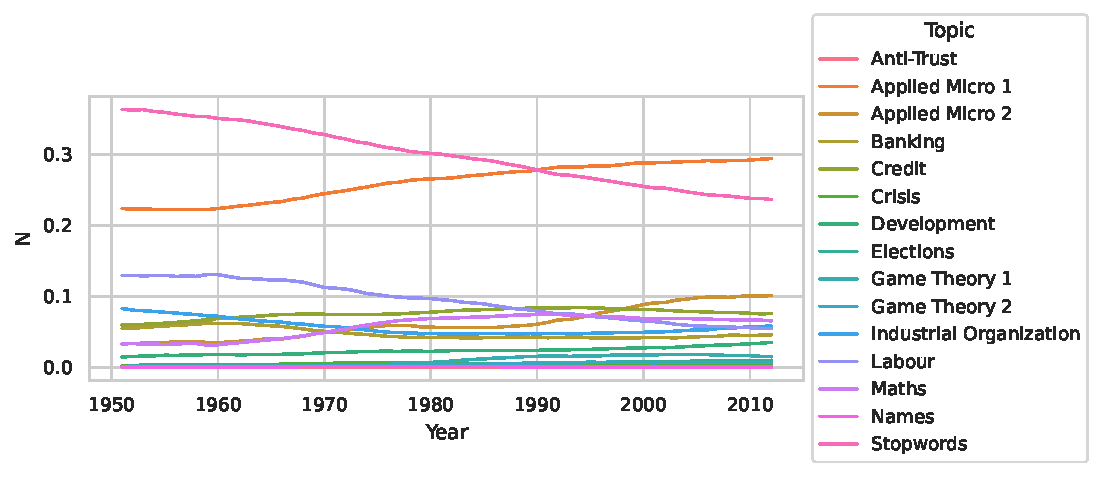
\includegraphics[width=\textwidth]{src/topics.pdf}
		\caption[Topics]{Prevalence of each topic during time. Smoothed with a 10-year rolling average}
	\end{figure}
\end{frame}

\section{Where is the mainstream pluralism?}

\begin{frame}
	\frametitle{Subgroups}
	\tiny \begin{table}[tb]
\caption[Subgroups]{The number of groups in the more detailed level of the hierarchy for each group in the level of interest}
\label{tab:subgroups}
\begin{tabular}{lr}
\toprule
\midrule
Industrial Organization & 10 \\
Game Theory – Auctions & 8 \\
Applied Micro & 6 \\
Macro 1 & 6 \\
Macro 2 & 6 \\
Macro Econometrics & 6 \\
Game Theory -  Theory & 5 \\
Game Theory – Elections & 5 \\
Labour & 5 \\
Trade & 4 \\
Econometrics & 2 \\
\bottomrule
\end{tabular}
\end{table}

\end{frame}

\begin{frame}
	\frametitle{Unique words}
	\begin{figure}
		\centering
		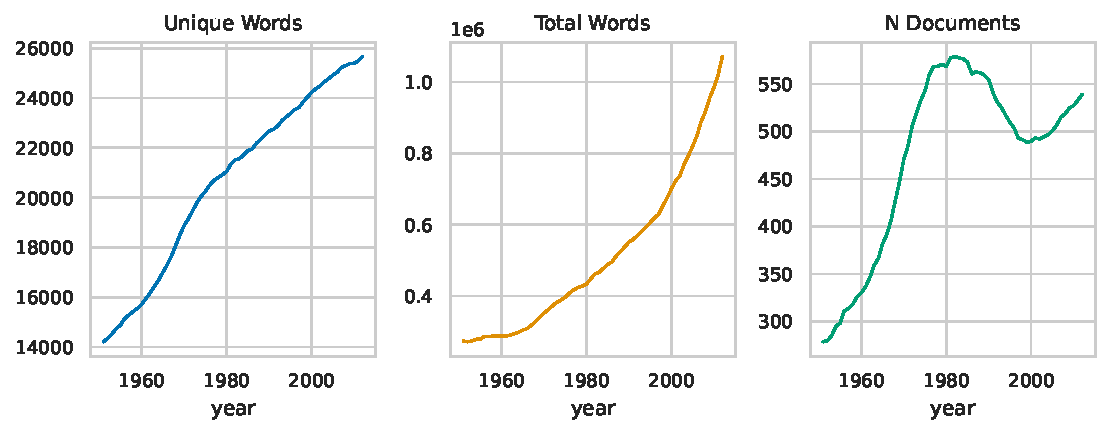
\includegraphics[width=\textwidth]{src/uwords.pdf}
		\caption[Unique Words]{From left to right: number of unique words per year in the sample; total number of words per year in the sample; number of documents per year in the sample}
	\end{figure}
\end{frame}

\begin{frame}
	\frametitle{Limitations}
	\begin{enumerate}
		\item No state-of-the-art algorithm (replicability and robustness problems)
		\item Are full-texts a source of information or noise? Are abstracts or titles a better data source?
		\item The timing of mainstream pluralism in the Top journals (after 2008? \~2015?)
		\item What signals are we looking for? How to measure them?
		\item Back to the theory!
	\end{enumerate}
\end{frame}

\section*{}
\begin{frame}
	\centering
	Thanks for your attention!

	Any question?
\end{frame}

\end{document}
